\section{Hardware Optimization}
\label{sec:hardware-optimization}

% 如何设计硬件以高效支持大模型的推理是一个挑战。这主要是由于大模型的arithmetic intensity和以前的各种任务都有很大差异，第一是LLM的decode阶段可能会有非常大的arithmetic intensity，第二是不同阶段，或者不同batchsize或者不同seqlength会有非常不同的arithmetic intensity。因此，设计硬件时需要非常仔细地考虑这些问题。本section中，我们将会从如何解决arithmetic intensity的问题的角度对LLM inference的硬件优化进行survey和分析。

Designing hardware to efficiently support inference for LLMs is a challenging task due to the varying arithmetic intensity\footnote{Arithmetic intensity refers to the ratio of arithmetic operations to memory access, which has been described in Roofline model (Section~\ref{sec:Rooflinemodel}).} under different inference stages and workload conditions. 
% significant differences in arithmetic intensity compared to previous tasks.
% This challenge arises primarily from one key factors: \textbf{Low Arithmetic Intensity during Decoding}:
Specifically, the prefill stage usually leverages GEMM operators to process the batched tokens, which exhibits high arithmetic intensity. On the contrary, the decoding stage calculates output tokens one at a time, which necessitates the use of either GEMV operators or lean GEMM operators to process the attention and FFN layers. These operators are characterized by low arithmetic intensity.  
% arithmetic operations compared to the large amount of memory access required (weight and KV cache), leading to a low 
% arithmetic intensity. 


% \textbf{Variability in Arithmetic Intensity}: 
% The arithmetic intensity can vary greatly across prefill/decode stages, 
Furthermore, the arithmetic intensity can exhibit substantial variation depending on the batch sizes and sequence lengths. For instance, a large batch size could significantly alter the arithmetic intensity, and a long sequence length may increase the memory access overhead of  KV-cache reading in each decoding step. This variability introduces additional complexity into the hardware design process, as different stages or configurations may necessitate distinct optimization strategies. Hence, it's crucial to consider these factors when designing hardware to ensure efficient performance across a wide range of scenarios.

Considering these challenges, careful consideration and optimization of hardware designs are necessary. In this section, we will survey and analyze various hardware optimizations  tailored for efficient LLM inference, with a focus on addressing the issues related to varying arithmetic intensity.

\subsection{Spatial Architecture}

% 由于LLM的decode过程是自回归的，因此在常用的对话等任务中LLM infernece大部分的时间都会花到decode阶段。因此一个关键的问题是如何解决The problem of low arithmetic intensity during decoding arises from a large number of memory accesses to both weights and the KV cache. 有一系列的工作提出使用Spatial Architecture来将不同的计算单元组织起来，每个单元都能有独立的memory access能力，从而整体上提升了系统的bandwidth上限。

The decoding process of LLM involves predicting words one at a time based on previously generated ones. However, this process can be costly, especially during tasks in long sequence generation. This is because the model needs to access large amount of weights and the key-value (KV) cache to generate each token, resulting in low arithmetic intensity.


There are several solutions that have been developed to address this issue. One such solution is the implementation of a "Spatial Architecture". In contrast to traditional computer architectures, spatial architectures utilize a different approach to computing. Instead of folding the computation process into multiple interactions between processing elements (PEs) and main memory, spatial architectures distribute the computation across multiple PEs. This design allows for the exploitation of parallelism, as each PE simultaneously performs a portion of the computation. Additionally, the intermediate data flows between the PEs, avoiding writing back to DRAM each time.
% It is important to consider the connectivity between the PEs when designing the overall computation flow.

\begin{figure}[t]
    \centering
    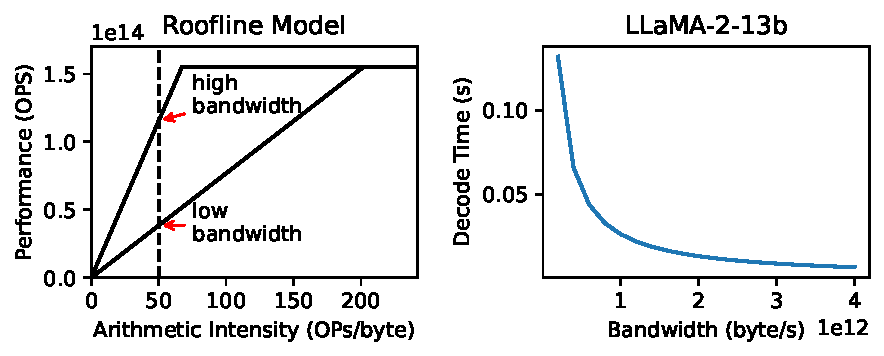
\includegraphics[width=0.95\linewidth]{ims/hardware_bandwidth.pdf}
    % \vspace{-0.6in}
    \caption{Effect of bandwidth on roofline model and Llama-2-13b. (Batch size=1, sequence length=1024)}
    \label{fig:hardware_bandwidth}
\end{figure}

In a spatial architecture, each PE is responsible for a specific portion of the computation. To facilitate efficient communication, data is typically moved between neighboring PEs. This allows for improved performance and efficient utilization of resources.
In a spatial setup, each PE has its own direct access to memory. This enables multiple processing units to access memory simultaneously, improving the overall speed at which information can move in and out of memory. This results in enhanced memory bandwidth and overall LLM inference performance.
As shown in Figure~\ref{fig:hardware_bandwidth}, as the total memory bandwidth increase, the performance for the linear layer in decoding stage can significantly increase.

In one case, Groq employs their LPU~\citep{abts2022groq_lpu} to create a spatial system for LLM inference. This system achieves a remarkable speed of over 300 tokens per second per user on the Llama-2-70b model~\citep{groq2023lpu_report}. Another example is Graphcore's Intelligence Processing Unit (IPU), which is another type of spatial architecture that efficiently executes LLMs~\citep{graphcore_gradient_huggingface}.



% Several solutions have been thought up to help with this. One approach is to organize the computing parts in a special way. This is called a "Spatial Architecture". 
% Unlike traditional computer architectures that rely on sequential execution and a central processing unit (CPU), spatial architectures aim to exploit parallelism by distributing computation across multiple processing elements. Each processing element is responsible for a specific portion of the computation, and data is typically moved between neighboring processing elements to enable efficient communication.
% Spatial architectures can be explicitly programmed to define the behavior and interaction of the processing elements. Programming models for spatial architectures often involve specifying data dependencies and communication patterns between processing elements, allowing programmers to exploit parallelism and optimize performance.
% In a spatial setup, each processing unit (PE) has its own direct access to memory. This means different processing units (PE) can access at the same time. It improves the total memory bandwidth, or overall speed that information can move in and out of memory.

% By handling memory traffic better, a spatial design may help address the low "arithmetic intensity" issue seen in decoding. Arithmetic intensity refers to how much number calculation is done versus how much time is spent accessing memory. More independent memory access through a spatial setup could boost this intensity and the overall decoding speed for conversations.


\subsection{Processing in Memory}

The decoding phase of LLM inference experiences the so-called "Memory Wall" problem, primarily due to its low arithmetic intensity. This issue is not new, the computer architecture community has been struggling with the "Memory Wall" problem for several decades. Among various potential solutions, processing in-memory  techniques (PIM) have garnered significant interest in recent years. By placing compute units directly in memory chips, we can leverage the much higher internal memory bandwidth and reduce the data movement overhead between memory and CPU/GPU cores. 
% This technique is called Near-Memory Computing (NMC).
% For instance, Samsung has released its HBM PIM product and   
% Sk-hynix has released its GDDR PIM.

In recent years, DRAM-based PIM has entered the commercialization phase, which can potentially mitigate the memory bandwidth bottleneck of LLM inference. As listed in Table~\ref{tab:pim-compare}, UPMEM's PIM-DIMM~\cite{upmem} is the first commercialized DRAM-PIM product, which places general-purpose RISC cores in DDR4-DIMMs. However, this product was not intended for deep-learning applications, thus the peak bandwidth and throughput can hardly meet the requirements of LLM inference. Compared to UPMEM's PIM-DIMM, Samsung proposes to place MAC units into HBM memory, achieving 2TB/s of internal memory bandwidth, which is much higher than that of traditional HBM2 (307GB/s per cube) memory. Since the processing units are tailored for deep learning workloads, the peak compute throughput of HBM-PIM can reach 1.2TFLOPS. In other words, HBM-PIM is suitable for accelerating operators with 1-2 Ops/Byte of arithmetic intensity. 

 Choi et al has proposed to accelerate the KV-Cache processing using HBM-PIM, which has low arithmetic intensity in batched LLM inference. According to their evaluation~\cite{choi2023unleashing}, A GPU+HBM-PIM system for LLM inference can achieve 3.24$\times$ speedup over traditional  monolithic GPU system. 

 

Similar to Samsung's HBM-PIM, SK-hynix has also proposed a GDDR6-based PIM accelerator~\cite{gddr-pim} called AiM. As shown in Table~\ref{tab:pim-compare}, the compute units of AiM adopts the BF16 data format, which is more efficient for deep-learning acceleration. With optimized MAC units, AiM offers 1TFLOPS per chip of compute capacity, while the peak bandwidth is 1TB/s per chip. Although AiM has not reported its performance on LLM, it can achieve up to 10$\times$ speed improvement compared to GPU+HBM2 system on LSTM tasks. 

Note that, although DRAM-based PIM techniques have demonstrated promising potential of  accelerating memory-intensive operators in LLM inference, there are still some limitations that should be addressed in the future. 

\begin{itemize}
\item \textbf{Limited Computation Power.} A key restriction of DRAM-PIMs in accelerating LLMs  stems from their constrained computational capabilities. DRAM-PIMs utilize compute units crafted using the DRAM process, resulting in transistors that are 3 times slower and logic density several times lower compared to CMOS in the same technology node~\cite{devaux2019true}. Even worse, DRAM chips usually have fewer metal layers, leading to a lower routing density at the same time. Due to these technical constraints, DRAM-PIMs can hardly incorporate powerful compute units. As a consequence, DRAM-PIMs is only suitable for small-batch inference or KV-cache processing. For computation-intensive large-batch inference, a powerful host is still necessary.

\item \textbf{Capacity Constraints.} Another significant limitation of DRAM-PIMs is their restricted capacity. Given that DRAM-PIMs allocate some memory capacity to construct the computation units, the total memory capacity is typically 50\% less than that of standard memory~\cite{hbm-pim}. For LLM applications that necessitate substantial memory capacity to accommodate the weights and KV-cache, DRAM-PIMs may encounter capacity-related challenges.

   \item \textbf{Inadequate Inter-PIM Communication.} In addition to the constraints imposed by computation power and capacity, another limitation of DRAM-PIMs  is their suboptimal inter-PIM communication capability. Given that there are distributed computing units located near each DRAM bank, data aggregation and computation synchronization among these units are unavoidable. However, DRAM-PIMs lack robust interconnects~\cite{zhou2023dimm,jonatan2024scalability}, and they typically depend on the host CPU/GPU for data exchange between PIM units. This reliance can lead to inefficiencies in the system. Therefore, to enhance LLM inference, future iterations of DRAM-PIMs should aim to improve their inter-PIM communication abilities.
\end{itemize}



 
\begin{table}[t]
\centering
\caption{Comparison of Commodity DRAM NMC Products}
\label{tab:pim-compare}
\resizebox{0.475\textwidth}{!}{
\begin{tabular}{|c|c|c|c|}
\hline
Product         &  PIM-DIMM & HBM-PIM          & AiM            \\ \hline
Technique  &       DDR4         & HBM2   & GDDR6  \\ \hline
PIM Units &  RISC Cores   & FP16 MAC   &  BF16 MAC      \\ \hline
Peak Bandwidth  &   80.4 GB/s    per DIMM          & 2 TB/s per cube   & 1 TB/s per chip  \\ \hline
Peak Throughput &   43.8 GOP/s per DIMM             & 1.2 TFLOPS & 1 TFLOPS \\ \hline
%  Arithmetic Intensity        &         0.54 OP/Byte       & 0.6 OP/Byte           & 1 OP/Byte          \\ \hline
\end{tabular}
}
\end{table}


% LPDDR PIM, 
% CXL PIM. 

% Process-in-Memory (PIM) is another emerging technology that has potential to address the challenges associated with the inference of LLMs and other data-intensive workloads. 
% Traditional von Neumann architectures, where data is transferred between the processor and memory, can become a bottleneck for these computationally intensive tasks. 
% PIM technology aims to mitigate this bottleneck by bringing the computation into to the memory, eliminating the data access as large as possible.
% PIM architectures integrate processing units directly into memory chips or memory modules.
% This allows computation to be performed within the memory itself, reducing the need for data movement between the processor and memory.
% With LLMs, we can store weights in the memory and input activation data to execute multiplication-and-accumulation (MAC) in the linear layer. 
% This reduces latency and energy consumption associated with data transfer, resulting in improved performance.

% Although PIM and NMC are still in early stages and face challenges in programming models, memory organization, and architectural design, they show promise in solve the problem of "Memory Wall", enhancing the performance and energy efficiency of LLM inference.

% \subsection{Sparse Support}

\subsection{New Data Format}
\label{sec:dataformat}

% intro: FP/Uniform/Non-uniform vs. Precision/Range/Efficiency/Friction

% As discussed in sec \ref{sec:quantization}, quantization casts individual tensor values from high-resolution floating-point (e.g. BF16, FP32) to low-resolution data types (e.g. INT4, INT8).
% At the expense of acceptable tuning effort and minor numerical accuracy degradation, tensor operations in the quantized models can be efficiently implemented on hardware.
% The diversity of underlying quantization formats, along with quantization algorithms and hardware implementations, render a vast and complex design space, which introduces nuanced and intricate trade-offs between numerical accuracy, tuning effort, and hardware efficiency.
Neural networks typically employ high-precision floating-point numbers (16 or 32 bits) for training. While high-precision FP numbers can accommodate both representation precision and range, the complex hardware implementation required for FP arithmetic is not conducive to efficient inference.
To mitigate the hardware overhead, uniform quantization casts high-precision floating-point numbers to low-precision integer representations, substituting expensive floating-point logic with efficient integer logic. However, uniform quantization struggles to balance representation precision and range simultaneously, leading to substantial degradation in model accuracy. 
Moreover, preserving model accuracy without degradation necessitates well-designed quantization algorithms, introducing additional casting efforts.
Non-uniform quantization attempts to enhance the precision of data representation under low-bit conditions by assigning bits and discretizing the range of parameters non-uniformly. Yet a critical drawback of non-uniform quantization is its challenging deployment on general computation hardware, e.g. CPUs and GPUs~\citep{gholami2022survey}.
In summary, existing data formats fail to concurrently achieve fine precision, extensive range, high efficiency, and low tuning costs for inference.
Given the criticality of reducing the deployment costs of LLMs, a substantial amount of work investigate into exploring the most balanced data format tailored to LLMs.

\begin{table}[htbp!]
\centering
\resizebox{\linewidth}{!}{%
\begin{tabular}{cccc}
    \hline
    \textbf{Aspect} & \begin{tabular}{@{}c@{}} \textbf{Floating} \\ \textbf{Point} \end{tabular} & \begin{tabular}{@{}c@{}} \textbf{Uniform} \\ \textbf{Quantization} \end{tabular} & \begin{tabular}{@{}c@{}} \textbf{Non-Uniform} \\ \textbf{Quantization} \end{tabular} \\
    \hline
    Precision        & Good & Bad & Medium \\
    Range            & Good & Bad & Medium  \\
    HW Efficiency    & Bad  & Good & Bad  \\
    Casting Effort    & Good  & Bad & Medium  \\
    \hline
\end{tabular}
}
\caption{Comparison of Floating Point, Uniform Quantization, and Non-Uniform Quantization}
\label{tab:data_format_comparison}
\end{table}

% Industrial efforts
To trade for better hardware efficiency from the original FP model, a natural progression is to reduce the exponent \& mantissa bits in the high-resolution floating-point format.
As demonstrated by recent works~\citep{micikevicius2022fp8, sun2019hybrid}, models of various categories pre-trained in FP16 (including LLMs) can be directly quantized to FP8 without significant accuracy degradation. Moreover, on a wide spectrum of tasks, training with FP8 can effectively match the result quality achieved by 16-bit training sessions.
The significant gain of hardware efficiency and little demand of user efforts envisioned by low-resolution float-point formats have garnered the attention from AI hardware manufacturers.
For instance, NVIDIA implements FP8 Tensor Core in their latest H100 GPUs~\citep{nvidiahopperarchitecture}.
Tesla also introduces configurable floating point format, namely CFloat8, in their Tesla Dojo chip~\citep{tesladojotechnology}.

Beyond the noval architectures introduced by the industry, academia has also initiated efforts to exploiting the potential of low-precision floating-point format on LLMs.
ZeroQuant-FP~\citep{wu2023zeroquant} proposes FP4 and FP8 for weight/activation quantization of LLMs. The authors adopt scaling constraints for weight quantization, achieving efficient weight conversion from FP4 to FP8 and better utilization of the FP8 Tensor Core.
ZeroQuant-(4+2)~\citep{wu2023zeroquant1} and FP6-LLM~\citep{xia2024fp6} proposes weight quantization of LLMs with FP6, and provides efficient implementation on CUDA Core and Tensor Core, respectively. 
% TODO: ZeroSpeed FP6
LLM-FP4~\citep{liu2023llm} proposes quantizing both weights and activations of LLMs down to FP4.
In summary, these efforts demonstrates the feasibility of applying floating-point formats at even lower bit-widths for quantization, as well as the potential for achieving greater efficiency gains on existing or new hardware platforms.

% More Intra-value adaptivity: Dynamic-length encoding
On the other hand, researchers are delving into the refinement of low-precision quantization formats to augment the adaptability of data representation whilst preserving hardware efficiency. 
One line of works propose to explore new encoding schemes within single value representation.
Contrary to INT and FP numbers, which utilize fixed-length sub-fields for encoding distinct pieces of information, such as exponents and mantissas, the newly-proposed rule-based quantization formats enable dynamic adjustment of sub-field bit-widths. 
ALPS~\citep{langroudi2021alps} proposes a generalized posit format along with a new adaptive quantization algorithm to optimally represent the dynamic range and distribution of DNN parameters.
ANT~\citep{guo2022ant} proposes a new data format called flint with leading-1 encoding for exponent fields.
Dybit~\citep{zhou2023dybit} proposes to separate exponent and mantissa fields with the first encountered 0 as delimiter.
The flexibility of these variable-length data formats presents the chance to compromise between range and precision more effectively and allows for customization to more closely align with the distribution of LLMs' weights and activations.

% Inter-value adaptivity: block-level representation, outlier-aware quantization
Another line of works exploit similarity and discrepancy across values.
Outlier-aware quantization capitalizes on the observation that values with large magnitudes have a significant impact on model performance. In this approach, important values are identified as outliers and are treated differently from normal values to ensure a more accurate representation. 
OLAccel~\citep{park2018energy} and GOBO~\citep{zadeh2020gobo} separately store and allocate higher bit-width to the outlier values.
OliVe~\citep{guo2023olive} refines the concept with outlier-victim pair encoding scheme to ensure aligned memory access and improved efficiency.
Bit-sharing encoding concentrates on the inherent similarity among values and annotates additional information in coarse granularity, thereby achieving a balance between representation accuracy and hardware efficiency. 
AdaptivFloat~\citep{tambe2020algorithm} proposes to optimally shift the available range of FP values with a common tensor-wise exponent bias.
MX~\citep{darvish2023shared} extends AdaptivFloat's observation into finer granularity, and proposes Block Data Representation (BDR) framework to explore the optimal tradeoff between representation accuracy and hardware efficiency.

\begin{table}[htbp!]
\centering
\resizebox{\linewidth}{!}{%
\begin{tabular}{ccc}
    \hline
    \textbf{Method} & \textbf{Description} & \textbf{Benefits} \\
    \hline
    Low-bit floating-point & Reduce exponent \& mantissa bits & Efficiency $\uparrow$ \\ 
    Variable-length encoding & Dynamically adjust sub-field bit-width & Precision $\uparrow$ \\
    Outlier-aware quantization & Customize quantization for outliers & Precision $\uparrow$ \\ 
    Bit-sharing encoding & Share common information within a block & Precision $\uparrow$ \\ 
    \hline
\end{tabular}
}
\caption{Summary of improvements in data formats. The benefits comes with negligible negative impacts on other factors.}
% \label{tab:data_format_comparison}
\end{table}

\subsection{New Processing Element}

% New processing element (PE) architectures for large languages models, such as transformer engine in nvidia GPU, GOBO, FPGA.

Except for the high demand for memory access, there has been a growing interest in developing specialized processing elements (PEs) to boost the computation. 
These specialized architectures aim to provide significant computational enhancements over general-purpose processing element, such as CUDA core, for the specific operations associated with LLMs.

NVIDIA has developed a special hardware acceleration engine called the Transformer Engine in their H100 GPU. This engine uses statistical analysis to determine the optimal precision (FP16 or FP8) for each layer of the model, achieving the best performance while maintaining accuracy.
Some researchers have designed accelerators specifically for efficiently executing the attention mechanism in language models (LLMs)~\citep{kao2023flat,qin2023fact}.
Several companies and research groups have been exploring the use of FPGAs to speed up LLM computations. Examples include DFX~\citep{hong2022dfx} and LightLLM~\citep{zeng2024flightllm}.

% For instance, NVIDIA has introduced a dedicated hardware acceleration engine called the Transformer Engine within their H100 GPU. 
% Transformer Engine 使用每层统计分析来确定模型每一层的最佳精度（FP16 或 FP8），在保持模型精度的同时实现最佳性能。
% Some work designed the accelerator for efficiently execute attention mechanism in LLMs~\citep{kao2023flat,qin2023fact}
% Several companies and research groups have been exploring the use of FPGAs for accelerating LLM computations, such as DFX~\citep{hong2022dfx} and LightLLM~\citep{zeng2024flightllm}.
% FPGAs offer flexibility in designing custom dataflow architectures tailored to the specific computational patterns of transformer models. 
% By mapping the parallelizable computations of LLMs onto the reconfigurable fabric of FPGAs, researchers have demonstrated significant performance gains and energy efficiency improvements compared to traditional CPUs and GPUs.